\chapter{Preparing the Sources}
\label{user-sources}

This chapter explains how to specify the source files that form the
basis of an analysis project, and describes options that influence parsing.

\section{Overview of source processing in \FramaC}\label{sec:overview}

For small projects and tests, processing the sources in \FramaC is as simple
as running \texttt{frama-c *.c}. For more complex projects, however,
some problems may arise when using this command, and the user must be aware
of the several steps involved in \FramaC source processing to fix them.

The diagram in Figure~\ref{fig:source-preparation} presents an overview
of the steps described in this chapter. For comparison purposes, we add
the equivalent process performed by a compiler such as GCC.

\begin{figure}[htbp]
  \begin{center}
    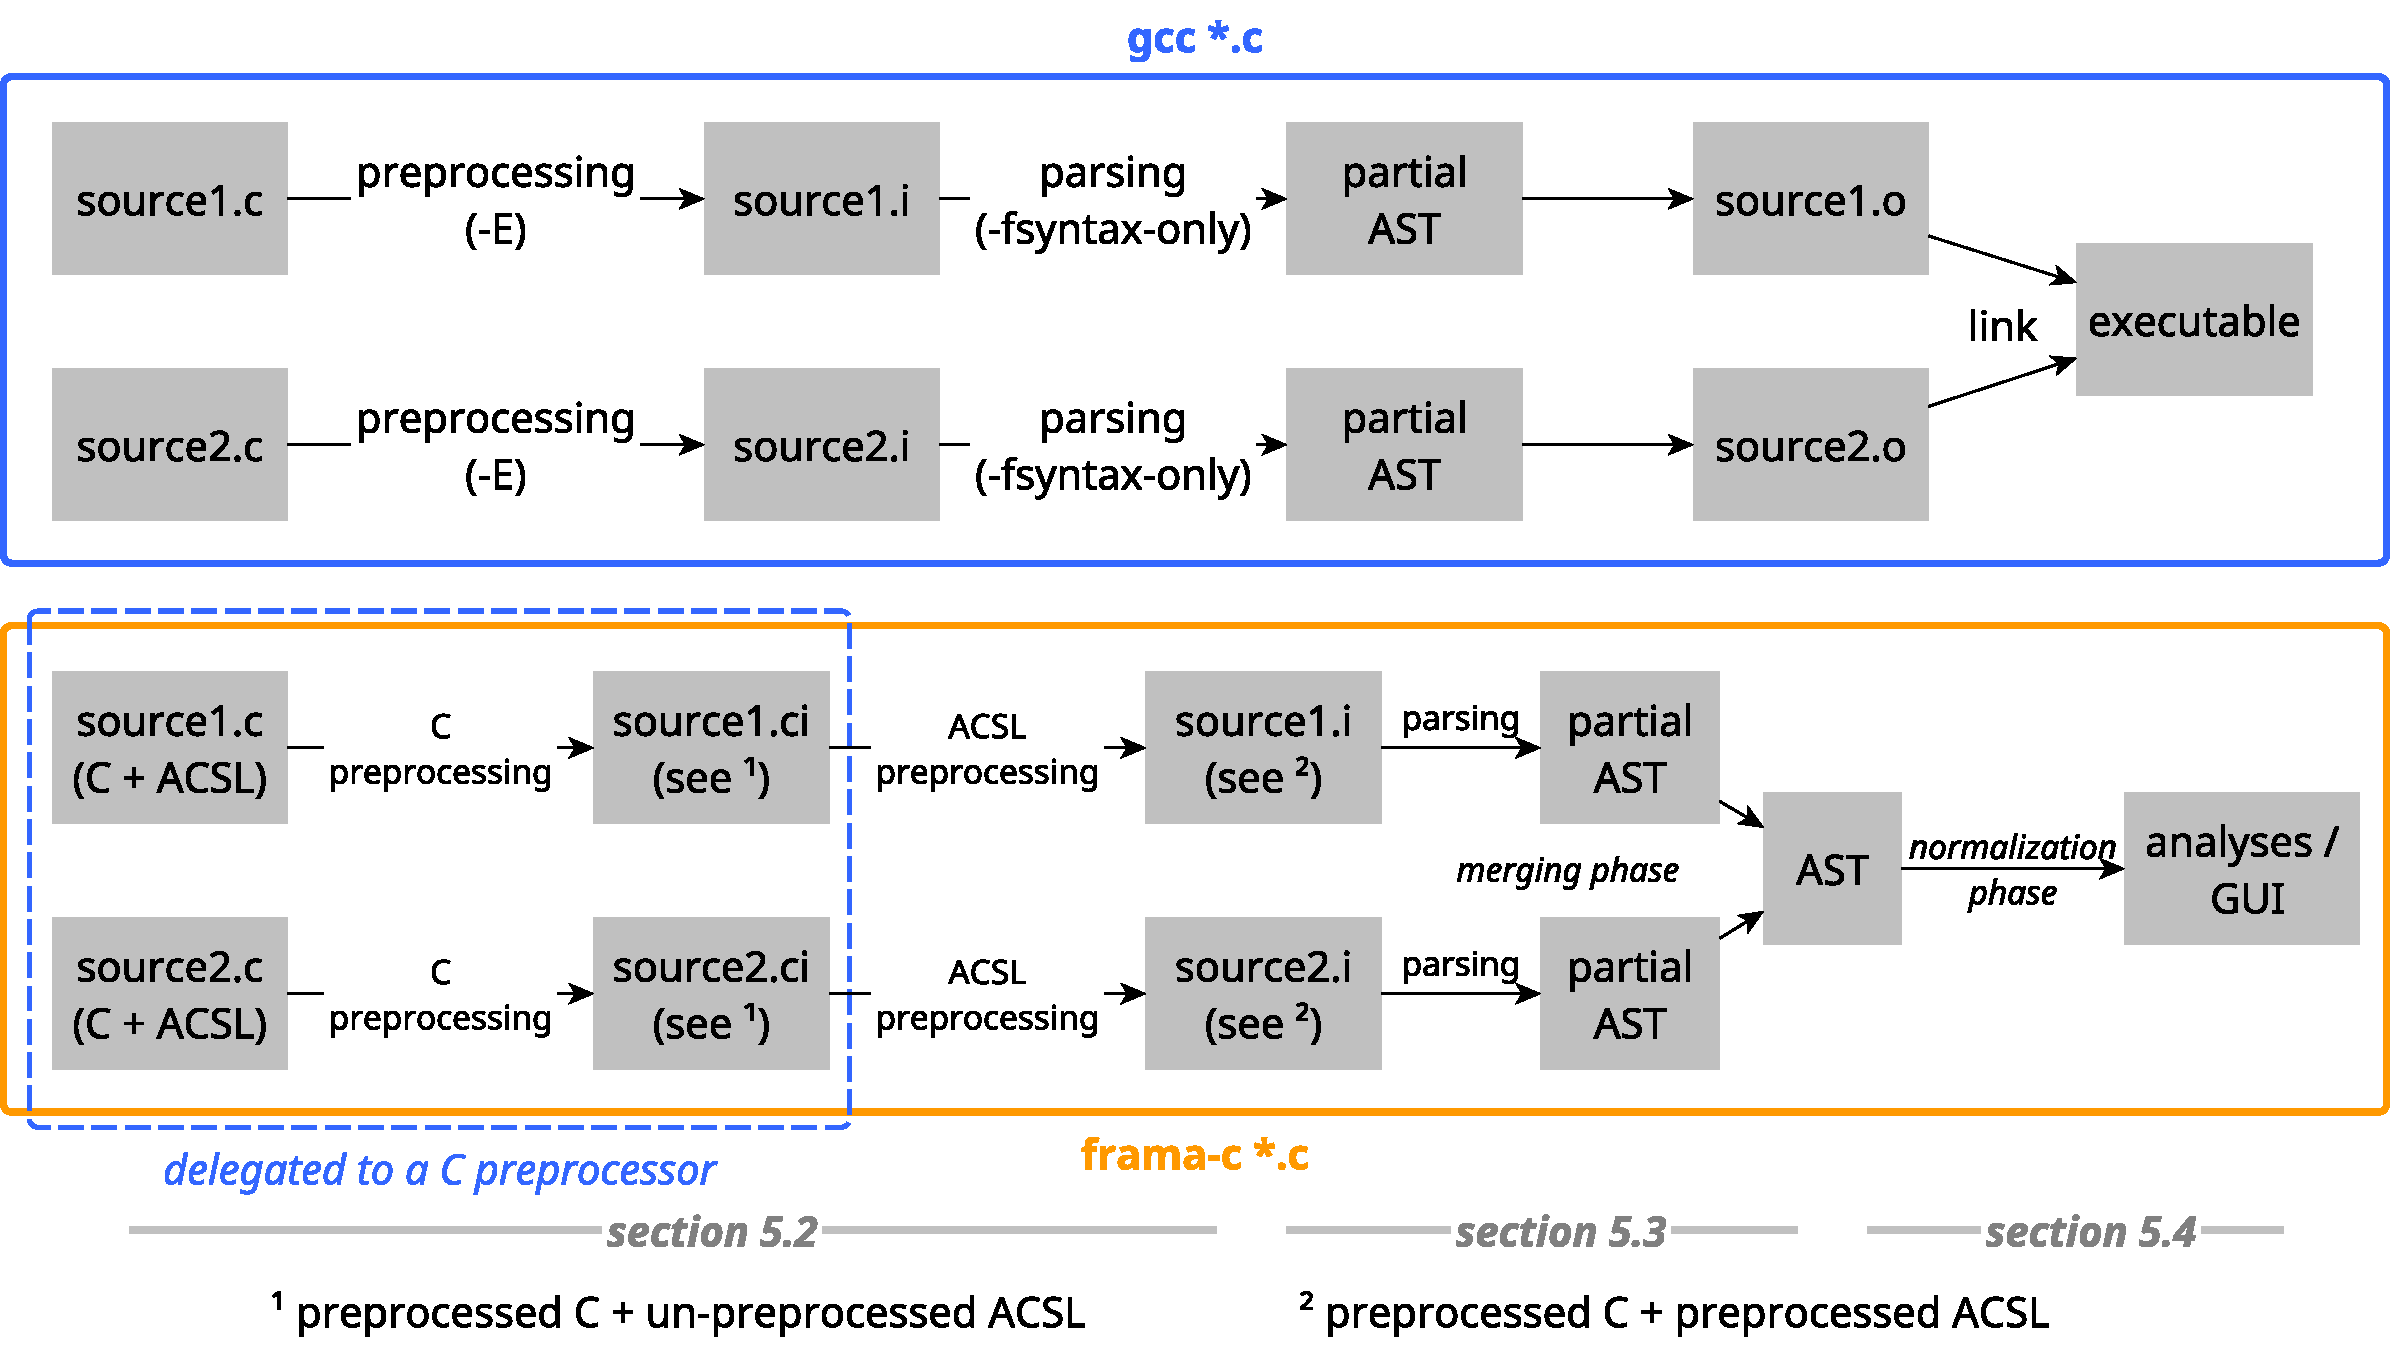
\includegraphics[width=\textwidth]{source-preparation.pdf}
    \caption{Overview of source preparation steps: as performed by GCC
      (top) and as performed by \FramaC (bottom).}
    \label{fig:source-preparation}
  \end{center}
\end{figure}

The following sections describe various options related to the steps shown
in the figure. Note that some plug-ins, such as \textsf{Variadic}
(described in chapter~\ref{user-variadic}), perform further AST
transformations before most analyses are run.

\section{Preprocessing the Source Files}\label{sec:preprocessing}

The list of files to analyze must be provided on the command line, or
chosen interactively in the GUI. Files with the suffix
{\tt .i} are assumed to be already preprocessed \C files. \FramaC
preprocesses {\tt .c} and {\tt .h} files with the following basic command:
\begin{shell}
\$ gcc -C -E -I .
\end{shell}
Plus some architecture-dependent flags. The {\em exact} preprocessing command
line can be obtained via options \texttt{-kernel-msg-key pp} and
\optiondef{-}{print-cpp-commands} (the latter exits \FramaC after printing).

Option \optiondef{-}{cpp-extra-args} can be used to add arguments to the
default preprocessing command, typically via the inclusion of defines
(\texttt{-D} switches) and header directories (\texttt{-I} switches), as in
\texttt{-cpp-extra-args="-DDEBUG -DARCH=ia32 -I./headers"}.
You can also add arguments on a per-file basis, using option
\optiondef{-}{cpp-extra-args-per-file}.

If you need to, you can also {\em replace} the preprocessing command
entirely with option \optiondef{-}{cpp-command}. Placeholders (see below)
can be used for advanced commands.
If no placeholders are used, the preprocessor is invoked in the
following way.
\begin{commands}
\texttt{<cmd> <args> <input file> -o <output file>}
\end{commands}

In this command, \texttt{<output file>} is a temporary filename chosen by
\FramaC while \texttt{<input file>} is one of the filenames provided by the
user.

For commands which do not follow this pattern, it is also possible to use
the following placeholders:

\begin{tabular}{|l|l|}
\hline
\texttt{\%input}, \texttt{\%i} or \texttt{\%1} & Input file \\
\hline
\texttt{\%output}, \texttt{\%o} or \texttt{\%2} & Output file \\
\hline
\texttt{\%args} & Additional arguments (see \texttt{-cpp-extra-args} below)\\
\hline
\end{tabular}

Here are some examples for using this option.
\begin{frama-c-commands}
\$ frama-c -cpp-command 'gcc -C -E -I. -x c' file1.src file2.i
\$ frama-c -cpp-command 'gcc -C -E -I. %args -o %o %i' file1.c file2.i
\$ frama-c -cpp-command 'cp %i %o'  file1.c file2.i
\$ frama-c -cpp-command 'cat %i > %o' file1.c file2.i
\$ frama-c -cpp-command 'CL.exe /C /E %args %i > %o' file1.c file2.i
\end{frama-c-commands}

When using \optionuse{-}{cpp-command}, you may add \optiondef{-}{cpp-frama-c-compliant}
to indicate that the custom preprocessor accepts the same set of options as GNU
\texttt{cpp}.
\optionuse{-}{cpp-frama-c-compliant} also implies some extra
constraints, such as accepting architecture-specific flags, e.g. \texttt{-m32}.

If you have a JSON compilation database file\footnote{%
  \url{http://clang.llvm.org/docs/JSONCompilationDatabase.html}}, you can use
it to retrieve preprocessing macros such as \texttt{-D} and \texttt{-I}
for each file in the database, via option
\optiondef{-}{json-compilation-database} \texttt{<path>}, where \texttt{<path>}
is the path to the JSON file or to a directory containing a
file named \texttt{compile\_commands.json}. With this option set,
\FramaC will parse
the compilation database and include associated preprocessing flags,
as if they had been manually added via \texttt{-cpp-extra-args-per-file}.
Note: if both \texttt{-cpp-extra-args-per-file} and the JSON compilation
database specify options for a given file, the former are used and the latter
are ignored. Also note that the use of the database simply adds flags
{\em for the files specified on the command-line}, but these files must still
be specified by the user.

In all of the above cases,
\acsl annotations are preprocessed by default (option \optiondef{-}{pp-annot}
is set by default). Unless a custom preprocessor is specified
(via \optionuse{-}{cpp-frama-c-compliant}), \FramaC considers that \gcc is
installed and uses it as preprocessor.
If you do \emph{not} want annotations to be preprocessed, you need to pass
option \texttt{-no-pp-annot} to \FramaC. Note that some headers in the
standard C library provided with \FramaC (described in Section~\ref{sec:libc})
use such annotations,
therefore it might be necessary to disable inclusion of such headers.

Also note that ACSL annotations are preprocessed separately from the C
code in a second pass, and that arguments given as \texttt{-cpp-extra-args} are
\emph{not} given to the second pass of preprocessing. Instead,
\texttt{-pp-annot} relies on the ability of \gcc to output all
macro definitions (including those given with \texttt{-D}) in the
preprocessed file. In particular, \texttt{-cpp-extra-args} must be
used if you are including header files who behave differently
depending on the number of times they are included.

In addition, files having the suffix \texttt{.ci} will be considered as needing
preprocessing for ACSL annotations only. Those files may contain
\texttt{\#define} directives and annotations are preprocessed as explained in
the previous paragraph. This allows to have macros in ACSL annotations while
using a non-GNU-like preprocessor.

\section{Merging the Source Code files}

After preprocessing, \FramaC parses, type-checks and links the source
code.  It also performs these operations for the \acsl annotations
optionally present in the program. Together, these steps form the
\emph{merging} phase of the creation of an analysis project.

\FramaC aborts whenever any error occurs during one of these steps. However
users can use the option
\texttt{-kernel-warn-key annot-error=active}\footnote{%
See section~\ref{sec:feedback-options} for more information on warning statuses.}
in order to
continue after emitting a warning when an \acsl annotation fails to type-check.

\section{Normalizing the Source Code}\label{sec:normalize}

After merging the project files, \FramaC performs
a number of local code transformations in the \emph{normalization} phase.
These transformations aim at making further work easier for the analyzers.
% VP: exclusively -> usually: it's not forbidden for a plugin to work on Cabs.
Analyses usually take place on the normalized version of the source code.
The normalized version may be printed by using
the option \optionuse{-}{print} (see Section~\ref{sec:io}).

The following options allow to customize the normalization process.
\begin{description}
\item \optiondef{-}{aggressive-merging} forces some function
  definitions to be merged into a single function if they are equal
  modulo renaming. Note that this option may merge two functions even
  if their original source code is different but their normalized
  version coincides. This option is mostly useful to share function
  definitions that stem from headers included by several source files.

\item \optiondef{-}{allow-duplication} allows the duplication of small
  blocks of code during normalization of loops and tests. This is set
  by default and the option is mainly found in its opposite form,
 \texttt{-no-allow-duplication} which forces \FramaC to use labels and
 gotos instead. Note that bigger blocks and blocks with a non-trivial
 control flow are never duplicated. Option \optionuse{-}{ulevel} (see
 below) is not affected by this option and always duplicates the loop body.

\item \optiondef{-}{annot} forces \FramaC to interpret \acsl annotations.
This option is set by default, and is only found in its opposite form
\texttt{-no-annot}, which prevents interpretation of
\acsl annotations.

\item \optiondef{-}{asm-contracts} tells \FramaC to generate \lstinline|assigns|
clauses for inline \lstinline|asm| statements using extended GNU notation
with output and input operands. This option is set by default, and opposite form
\texttt{-no-asm-contracts} prevents the generation of such clauses.
If the assembly block
already has a statement contract which is not guarded by a \lstinline|for b:|
clause \lstinline|assigns| clauses are generated only for behaviors which do not
already have one.

\item \optiondef{-}{asm-contracts-auto-validate} tells \FramaC to
automatically mark as valid \lstinline|assigns| clauses generated from
\lstinline|asm| statements. However, if an \lstinline|asm| statement contains
\lstinline|memory| in its clobber list, the corresponding clause will \emph{not}
be considered valid through this option.

\item \optiondef{-}{collapse-call-cast} allows, in some cases,
the value returned by
a function call to be implicitly cast to the type of the value it is
assigned to (if such a conversion is authorized by the C
standard). Otherwise, a temporary variable separates the call and the
cast. The default is to have implicit casts for function calls, so the
opposite form \texttt{-no-collapse-call-cast} is more useful.

\item \optiondef{-}{constfold} performs a syntactic folding of
constant expressions. For instance,
the expression \texttt{1+2} is replaced by \texttt{3}.

\item \deprecatedoptiondef{-}{continue-annot-error} \emph{Deprecated option.}
  Just emits a warning and discards the annotation when it fails to type-check,
  instead of generating an error (errors in \C are still fatal). This behavior
  is now managed by warning category (Section~\ref{sec:feedback-options})
\texttt{annot-error}, whose default status is ``abort''. Behavior of
\texttt{-continue-annot-error} can thus be obtained with
\texttt{-kernel-warn-key annot-error=active}, or even
\texttt{-kernel-warn-key annot-error=inactive} to silently ignore any ill-formed
annotations.

\item \texttt{\optiondef{-}{enums} <repr name>} specifies which representation
should be used for a given enumerated type. Namely, the C standard allows the use
of any integral type in which all the corresponding tags can be represented.
Default is \texttt{gcc-enums}. A list of supported
options can be obtained by typing:
\begin{frama-c-commands}
\$ frama-c -enums help
\end{frama-c-commands}
This includes:
\begin{itemize}
\item \texttt{int}: treat everything as \texttt{int} (including enumerated types
with \texttt{packed} attribute).
\item \texttt{gcc-enums}: use an unsigned integer type when no tag has a
negative value, and choose the smallest rank possible starting from \texttt{int}
(default \gcc's behavior)
\item \texttt{gcc-short-enums}: use an unsigned integer type when no tag has
a negative value, and choose the smallest rank possible starting from
\texttt{char} (\gcc's \texttt{-fshortenums} option)
\end{itemize}

\item \optiondef{-}{initialized-padding-locals} forces to initialize padding
  bits of locals to 0. If false, padding bits are left uninitialized. This
  option is set by default.

\item \texttt{\optiondef{-}{inline-calls} <f1,...,fn>} inlines calls to
  functions. Use \texttt{@inline} to select all functions with attribute
  \texttt{inline}.
  For recursive functions, only the first level
  is inlined (e.g., the function will contain an inlined version of itself with
  a recursive call inside it). Calls via function pointers are ignored.

\item \texttt{\optiondef{-}{remove-inlined} <f1,...,fn>} removes from the AST
  functions \texttt{f1,...,fn}, which must have been given to
  \optionuse{-}{inline-calls}. Note: this option does not check if the given
  functions were fully inlined.

\item \optiondef{-}{keep-switch} preserves \texttt{switch} statements in the
  source code. Without this option, they are transformed into \texttt{if}
  statements. An experimental plug-in may require this option to be unset
  to avoid having to handle the \texttt{switch} construct.
  Other plug-ins may prefer this option to be used because it better
  preserves the structure of the original program.

\item \optiondef{-}{keep-unused-specified-functions} does not remove from the
  AST uncalled function prototypes that have ACSL contracts. This option is
  set by default. So you mostly use the opposite form, namely
  \optiondef{-}{remove-unused-specified-functions}.

\item \optiondef{-}{keep-unused-types} does not remove unused types and
  enum/struct/union declarations. By default, such types are removed,
  that is, its opposite option \optiondef{-}{remove-unused-types} is set.

\item \texttt{\optiondef{-}{machdep} <machine architecture name>} defines the
  target platform. The default value is a \texttt{x86\_64} bits
  platform. Analyzers may take into account the \emph{endianness} of the
  target, the size and alignment of elementary data types, and other
  architecture/compilation parameters. The \texttt{-machdep} option provides a
  way to define all these parameters consistently in a single step.
  Note that multiarch preprocessors such as GCC's may require special flags
  to ensure compatibility with the chosen machdep, e.g. \texttt{-m32} for a
  \texttt{x86\_64} GCC compiling 32-bit code. In most cases this is handled
  automatically, but otherwise option \optionuse{-}{cpp-command} can be used.

The list of supported platforms can be obtained by typing:
\begin{frama-c-commands}
\$ frama-c -machdep help
\end{frama-c-commands}

Apart from these default platforms, it is possible to give as argument
to \texttt{-machdep} option the path of a YAML file containing the information
needed by \FramaC. The Plug-in Development Guide~\cite{plugin-dev-guide} describes
this format in more detail, as well as the use of the \texttt{make\_machdep.py}
script to automatically generate it. The YAML schema contains a list of builtin
macros with their values. However, any such \texttt{MACRO} can be undefined by passing
\texttt{-UMACRO} in the preprocessor arguments
(using \texttt{-cpp-extra-args} or its per-file counterpart as in Sect.~\ref{sec:preprocessing},
or a compilation database as in Sect.~\ref{sec:using-json-comp}). In addition,
since compilers tend to define builtin macros with a varying number of
underscores as prefix and suffix, \texttt{-UMACRO} will also undefine
\texttt{\_MACRO}, \texttt{\_\_MACRO}, \texttt{\_\_MACRO\_\_}, etc.

\item \optiondef{-}{simplify-cfg} allows \FramaC to remove break, continue and
  switch statements. This option is automatically set by some plug-ins that
  cannot handle these kinds of statements. This option is off by default.

\item \optiondef{-}{simplify-trivial-loops} simplifies trivial loops such as
  \texttt{do ... while(0)}. This option is set by default.

\item \texttt{\optiondef{-}{ulevel} <n>} unrolls all loops n times. This is a
  purely syntactic operation.  Loops can be unrolled individually, by
  inserting the \pragmadef{UNROLL} pragma just before the loop statement. Do
  not confuse this option with plug-in-specific options that may also be called
  ``unrolling''~\cite{value}. Below is a typical example of use.
\begin{ccode}
/*@ loop pragma UNROLL 10; */
for(i = 0; i < 9; i++) ...
\end{ccode}
The transformation introduces an \pragmadef{UNROLL} pragma indicating that the unrolling process has been done:
\begin{ccode}
... // loop unrolled 10 times
/*@ loop pragma UNROLL 10;
    loop pragma UNROLL "done", 10; */
  ... // remaining loop
\end{ccode}
That allows to disable unrolling transformation on such a loop when reusing \FramaC with a code obtained by a previous use of \FramaC tool.
To ignore this disabling \pragmadef{UNROLL} pragma and force unrolling, the option \texttt{\optiondef{-}{ulevel-force}} has to be set.

Passing a negative argument to \texttt{-ulevel} will disable unrolling, even
in case of \texttt{UNROLL} pragma.
\end{description}

\section{Normalizing Contracts}\label{sec:normalize-contracts}

Normalization gives a program which is semantically equivalent to the original
one, but there is an exception for function contracts. By default, function
contracts are left as is, but \FramaC and plug-ins can require the presence of
some specification to improve their performances. When they do, they can ask
\FramaC's kernel to generate specifications.

For example, let us say we have a function \texttt{f} that is only declared and
has no \acsl \texttt{assigns} clause, but these \texttt{assigns} are required by
\Eva. \Eva asks the kernel to generate \texttt{assigns} before resuming
the analysis. Indeed, as mentioned in the \acsl manual~\cite{acsl}, assuming
that \texttt{f} can write to any location in the memory would amount to stop any
semantical analysis at the first call to \texttt{f}, since nothing would be
known on the memory state afterwards.

The generation is done either by combining existing specifications or according
to a \emph{mode} which can be selected via \FramaC's options. A plug-in
developer has also the possibility to create their own mode using \FramaC's API.
The Plug-in Development Guide~\cite{plugin-dev-guide} describes all steps
required to create and use a custom mode. All available modes are detailed in
table~\ref{table:populate-mode}. Additionally, a status is emitted for each
generated clause. A summary can be found in table~\ref{table:populate-status}.

\begin{table}[t]
  \begin{minipage}{\linewidth}
    \begin{tabular}{@{}l|ll|ll|ll@{}}
      \multicolumn{1}{c|}{ \multirow{2}{*}{Mode}}
      & \multicolumn{2}{c|}{\texttt{ACSL}}
      & \multicolumn{2}{c|}{\texttt{Frama\_C}}
      & \multicolumn{2}{c}{\texttt{Safe}} \\

      & \multicolumn{1}{c}{Proto}  & \multicolumn{1}{c|}{Body}
      &  \multicolumn{1}{c}{Proto} & \multicolumn{1}{c|}{Body}
      &  \multicolumn{1}{c}{Proto} & \multicolumn{1}{c}{Body} \\ \midrule

      \texttt{exits}        & \multicolumn{1}{c}{-----}     & \multicolumn{1}{c|}{-----}
                            & \verb+\false+                 & \verb+\false+
                            & \multicolumn{1}{c}{-----}     & \verb+\false+ \\
      \texttt{assigns}      & \verb+\everything+            & \verb+\everything+
                            & Auto\footnote{Automatically generated using the function parameters.} & Auto
                            & \verb+\everything+            & \verb+\nothing+ \\
      \texttt{allocates}    & \verb+\nothing+               & \verb+\nothing+
                            & \texttt{ACSL}\footnote{Refer to \texttt{ACSL} mode to see what is generated.} & \texttt{ACSL}
                            & \verb+\everything+            & \verb+\nothing+ \\
      \texttt{terminates}   & \verb+\true+                  & \verb+\true+
                            & \texttt{ACSL}                 & \texttt{ACSL}
                            & \verb+\false+                 & \verb+\true+ \\
      \texttt{requires}     & \multicolumn{1}{c}{-----}     & \multicolumn{1}{c|}{-----}
                            & \texttt{ACSL}                 & \texttt{ACSL}
                            & \verb+\false+                 & \multicolumn{1}{c}{-----} \\
    \end{tabular}
  \end{minipage}
  \caption{Specification generation's behaviors according to available modes}
  \label{table:populate-mode}
\end{table}

By default, \FramaC selects the mode \texttt{Frama\_C} and the following options
allow selecting mode(s) for the specification generation:

\begin{description}
  \item \texttt{\optiondef{-}{generated-spec-mode <mode>}} selects which
  \texttt{mode} is used to generate missing specifications. \texttt{mode} can be
  either ``frama-c'', ``acsl'', ``safe'' or any custom mode registered in a
  plug-in.

  \item \texttt{\optiondef{-}{generated-spec-custom
  <clause\_1:mode\_1,clause\_2:mode\_2,...>}} has a similar behavior as
  \optionuse{-}{generated-spec-mode}, except that it allows the user choosing a
  \texttt{mode} individually for each clause. It also allows the user ignoring
  \FramaC and/or plug-ins needs by skipping the generation for a clause, with
  the mode ``skip''. This mode is not available with
  \optionuse{-}{generated-spec-mode} and trying to use it emits a warning and
  replaces it by \texttt{Frama\_C}. For example:
  \begin{frama-c-commands}
    \$ frama-c -generated-spec-custom exits:skip,requires:safe
  \end{frama-c-commands}
  Here every clause is generated using the default mode \texttt{Frama\_C} except
  for exits which are not generated and \texttt{requires} which are generated
  using the mode \texttt{Safe}.
\end{description}

As mentioned, the generation can also be done by combining existing clauses
from other behaviors following this algorithm:
\begin{itemize}
  \item[1.] If the function contract has some clauses \texttt{C} in unguarded
  (without \texttt{assumes} clauses) behaviors, we combine them in the default
  behavior.
  \item[2.] Else, if it has some clauses \texttt{C} in complete behaviors, we
  combine them in the default behavior.
  \item[3.] Else, if it has some clauses \texttt{C} anywhere, we combine them in
  the default behavior.
  \item[4.] Else we use the selected mode to generate these clauses (see mode's
  table).
\end{itemize}

{\em Note: There is an exception with the mode \texttt{ACSL} for which we never
try to combine existing clauses from other behavior, and jump directly to the
step of our algorithm to use the selected mode.}\\

\begin{table}[t]
  \centering
  \begin{tabular}{@{}l|l|l|l@{}}
      \multicolumn{1}{c|}{Mode} &
      \multicolumn{1}{c|}{\texttt{ACSL}} &
      \multicolumn{1}{c|}{\texttt{Frama\_C}} &
      \multicolumn{1}{c}{\texttt{Safe}} \\ \midrule

      \texttt{exits}      & Dont\_know                 & Dont\_know & Dont\_know \\
      \texttt{assigns}    & \multicolumn{1}{c|}{-----} & Dont\_know & Dont\_know \\
      \texttt{allocates}  & True                       & Dont\_know & Dont\_know \\
      \texttt{terminates} & True                       & Dont\_know & Dont\_know \\
      \texttt{requires}   & \multicolumn{1}{c|}{-----} & \multicolumn{1}{c|}{-----} & \multicolumn{1}{c}{-----} \\
  \end{tabular}
  \caption{Status emitted during the specification generation according to the selected mode}
  \label{table:populate-status}
\end{table}

When a clause is generated for a function, \FramaC's kernel can emit a warning
if this function is a prototype and if it is not part of \FramaC's builtins. The
message emitted depends on the generated clauses, their origins (if we combined
some clauses from existing ones, or generated them from nothing, or both) as
well as if the function contract was empty before the generation or incomplete.

\section{Incremental parsing} (experimental)\label{sec:incremental-parsing}

Parsing large code bases takes a non-negligible amount of time.
More importantly, non-modular analyses need to be recomputed in their entirety
even for minuscule AST changes.

In order to help deal with these issues, and to help support for future
incremental analyses (which recompute results only for the modified AST parts
and their dependencies), you can use option \optiondef{-}{ast-diff}.
It enables computing the difference between a previous AST (loaded via
option \verb|-load| (Section~\ref{sec:saveload}) and the AST computed from the
current sources. This difference is stored by the \FramaC kernel and can be
used by plug-ins which support it. Note however that since \verb|-load| implies that
files given on the command line are ignored, \verb|-load| and \verb|-ast-diff| with
the list of C files to consider must be properly sequenced through the use of
\verb|-then| or one of its variants (Section~\ref{sec:then}), as in:
\begin{frama-c-commands}
\$ frama-c -load previous.sav -then -ast-diff file1.c file2.c [...]
\end{frama-c-commands}

{\em Note: currently, parsing and type-checking are systematically performed
  even with this option, and \verb|-ast-diff| compares the normalized ASTs.
  In the future, though, these steps should be refactored to allow saving
  further time.}

\section{Predefined macros}\label{sec:predefined-macros}

\FramaC, like several compilers and code analysis tools, predefines and uses
a certain number of C macros. They are summarized below.

\begin{description}
\item \textttdef{\_\_FRAMAC\_\_}: defined to 1 during preprocessing by \FramaC,
as if the user had added \texttt{-D\_\_FRAMAC\_\_} to the command line. Useful
for conditional compilation and detection of an execution by \FramaC.

\item \textttdef{\_\_FC\_MACHDEP\_{\em XXX}}, where \texttt{{\em XXX}} is one of
  \texttt{X86\_16}, \texttt{X86\_32}, \texttt{X86\_64}, \texttt{PPC\_32} or
  \texttt{MSVC\_X86\_64}:
according to the option \optionuse{-}{machdep} chosen by the user,
the corresponding macro is predefined by \FramaC. Those macros correspond to
the values of \texttt{-machdep} that are built-in in the Frama-C kernel.
In addition, custom machdeps can be added
by plug-ins or scripts. If such a machdep named \texttt{custom-name}
is selected, \FramaC will predefine the macro
\texttt{\_\_FC\_MACHDEP\_CUSTOM\_NAME}, that is the upper-case version of the
name of the machdep.
Conversely, if an
\texttt{\_\_FC\_MACHDEP\_{\em XXX}} macro is defined by the user in
\texttt{-cpp-command} or \texttt{-cpp-extra-args}, then \FramaC
will consider it as a custom machdep and will {\em not} add any machdep-related
macros. It is then the responsibility of the user to ensure that
\texttt{-machdep} and \texttt{\_\_FC\_MACHDEP\_{\em XXX}} are coherent.

\item \textttdef{\_\_FC\_*}: macros prefixed by \texttt{\_\_FC\_} are reserved
  by \FramaC and should not be defined by the user (except for custom machdeps,
  as mentioned above, and for customization macros, as described below).
These include machdep-related macros and definitions
related to \FramaC's standard library.
\end{description}

Furthermore, some macros are undefined in the standard library, and can
be defined (e.g. through \lstinline|-cpp-extra-args|) to customize the \FramaC
standard library. They are described below.

\begin{description}
\item \textttdef{\_\_FC\_NO\_MONOTONIC\_CLOCK}: By default, \FramaC defines
  a \lstinline|MONOTONIC_CLOCK| in \lstinline|time.h|. If this macro is defined,
  this clock is not available.
\item \textttdef{\_\_FC\_INDETERMINABLE\_FLOATS}: By default, \FramaC's libc
  uses an IEEE-754 compatible environment. If this macro is defined,
  rounding mode and float evaluation
  (macros \lstinline|FLT_ROUNDS| and \lstinline|FLT_EVAL_METHOD|) will be
  considered as indeterminable.

\end{description}

\section{Compiler and language extensions}\label{sec:extensions}

\FramaC's default behavior is to be fairly strict concerning language features.
By default, most C99 and C11 features are accepted\footnote{For more details
about C99/C11 feature support, see
Section~\ref{sec:unsupported-iso-c-features}.}, but most non-ISO C compiler
extensions are not accepted, similarly to when compiling a program with
\verb+gcc -std=c11 -pedantic -pedantic-errors+.

However, depending on the machine architecture (see option
\optiondef{-}{machdep}, in Section~\ref{sec:normalize}),
\FramaC accepts some compiler extensions, namely for GCC and MSVC machdeps.
For instance, trying to parse a program containing an empty initializer,
such as \verb+int c[10] = {};+ will result in the following error message:

\begin{verbatim}
[kernel] user error: empty initializers only allowed for GCC/MSVC; see option
 -machdep or run 'frama-c -machdep help' for the list of available machdeps
\end{verbatim}

This means that using a GCC or MSVC machdep (e.g., \verb+-machdep gcc_x86_32+)
will allow the language extension to be accepted by \FramaC.

\section{Standard library (libc)}\label{sec:libc}

\FramaC bundles a C standard library in order to help parse and analyze code
that relies on the functions specified in the ISO C standard.
Furthermore, In order to simplify parsing of code using common open-source libraries,
\FramaC's standard library also includes some POSIX and non-POSIX headers which
are not part of ISO C.
Such libraries are provided on a best-effort basis, and they are part of the
{\em trusted computing base}: to ensure its correctness, the specifications
must be ultimately proofread by the user.

This library, while incomplete, is constantly being improved and extended.
It is installed in the sub-directory \texttt{libc} of the directory printed by
\texttt{frama-c -print-share-path}. It contains standard \C headers,
some \acsl specifications, and definitions for a few library functions.

By default, \FramaC's preprocessing will include the headers of its own standard
library, instead of those installed in the user's machine. This avoids issues
with non-portable, compiler-specific features.
Option \optiondef{-}{frama-c-stdlib} (set by default)
adds \verb+-I$(frama-c-config -print-share-path)/libc+ to the preprocessor command, as well as
GCC-specific option \texttt{-nostdinc}. If the latter is not recognized by
your preprocessor,
\optionuse{-}{no-cpp-frama-c-compliant} can be given to \FramaC
(see section~\ref{sec:preprocessing}).

The use of \FramaC's standard library contains a few caveats:
\begin{itemize}
\item definitions which are not present in \FramaC's standard library may cause
  parsing errors, e.g. missing type definitions, or missing fields in structs;
\item if a header is included which is not available in \FramaC's library,
  preprocessing will fail by default (due to the \texttt{-nostdinc} option);
  if the user manually includes the system's library, e.g. by adding
  \texttt{-cpp-extra-args='-I/usr/include'}, the preprocessor will end up
  mixing headers from \FramaC's library with those from the system, often
  leading to incompatible definitions and unexpected parsing errors.
  In this case, the best approach is usually to include {\em only} the missing
  definitions, for instance by copying them to a separate header file, included
  manually or via the GCC-compatible option \texttt{-include <header.h>}
  (see {\em GCC's Preprocessor Options} for more details). Alternatively,
  consider filing an issue (see Chapter~\ref{user-errors}) to ask for the
  inclusion of such headers and/or definitions in \FramaC's standard library.
\end{itemize}

Note that, while \FramaC's library intends to offer maximum portability, some
definitions such as numeric constants require actual values to be defined.
For pragmatic reasons, such definitions are most often based on the values
defined in GNU/Linux's libc, and may differ from those in your system.
As stated before, if you want to ensure the code analyzed by \FramaC is
strictly equivalent to the one from the target system, you must either
proofread the definitions, or provide your own library files.

\section{Warnings during normalization}\label{sec:warnings-normalize}

\emph{Note: the options below are deprecated, replaced by the more general and
  flexible mechanism of \emph{warning categories}, described in
  Section~\ref{sec:feedback-options}.}

Some options can be used to influence the warnings that are
emitted by \FramaC during the normalization phase.

\begin{description}
\item \texttt{\deprecatedoptiondef{-}{warn-decimal-float} <freq>}
  (\emph{deprecated}) warns
  when floating-point constants in the program cannot be exactly represented;
  freq must be one of \texttt{none}, \texttt{once} or \texttt{all}.
  Defaults to \texttt{once}.
  \emph{Superseded by warning category \texttt{parser:decimal-float}.}

\item \texttt{\deprecatedoptiondef{-}{implicit-function-declaration} <action>}
  (\emph{deprecated}) defines
  the action to perform (\texttt{ignore}, \texttt{warn} or \texttt{error})
  whenever a call to a function that has not been previously declared is found.
  This is invalid in C90 or in C99, but could be valid K\&R code.
  Defaults to \texttt{warn}.
  \emph{Superseded by warning category \texttt{typing:implicit-function-declaration}}.
  \textbf{Note:} parsing is not guaranteed to succeed, regardless of
  the emission of the warning. Upon encountering a call to an undeclared
  function, \FramaC attempts to continue its parsing
  phase by inferring a prototype corresponding to the type of the
  arguments at the call (modulo default argument promotions).
  If the real declaration does not match the
  inferred prototype, parsing will later end with an error.
\end{description}

\section{Testing the Source Code Preparation}

If the steps up to normalization succeed, the project is then ready for
analysis by any \FramaC plug-in. It is possible to test that the source code
preparation itself succeeds, by running \FramaC without any option.
\begin{frama-c-commands}
\$ frama-c <input files>
\end{frama-c-commands}

If you need to use other options for preprocessing or normalizing the source
code, you can use the option \optiondef{-}{typecheck} for
the same purpose. For instance:
\begin{frama-c-commands}
\$ frama-c -cpp-command 'gcc -C -E -I. -x c' -typecheck file1.src file2.i
\end{frama-c-commands}


% Local variables:
% mode: TeX
% TeX-master: "userman.tex"
% ispell-local-dictionary: "english"
% End:
